% Chapter Template

\chapter{Correct by Construction Agile Scrum Technique} % Main chapter title

\label{Chapter_Applying_the_methodology} % Change X to a consecutive number; for referencing this chapter elsewhere, use \ref{ChapterX}

We have now described the process we are going to follow. In this chapter, we describe 
the technique we are going to use the create the artefacts.

To create all the artefacts we need a mathematical specification language and a 
programming language.

\section{The system}
As an explanation aid we are going to consider an asynchronous data transfer
interface connecting a sender and receive.

\begin{figure}[H]
	\centering
	\includegraphics[scale=0.75]{Figures/AsyncInterface.pdf}
	\decoRule
	\caption{Asynchronous data transmission interface.}
	\label{fig:AsyncInterface}
\end{figure}

Data is sent on the \(value\) line, and the \(ready\) and \(acknowledge\) lines are
used for synchronization. The sender puts a value on the \(value\) line. The 
\(ready\) line is then switched (high to low, or low to high). When the receiver has
read the value the \(acknowledge\) is switched (high to low, or low to high).

\begin{figure}[H]
	\centering
	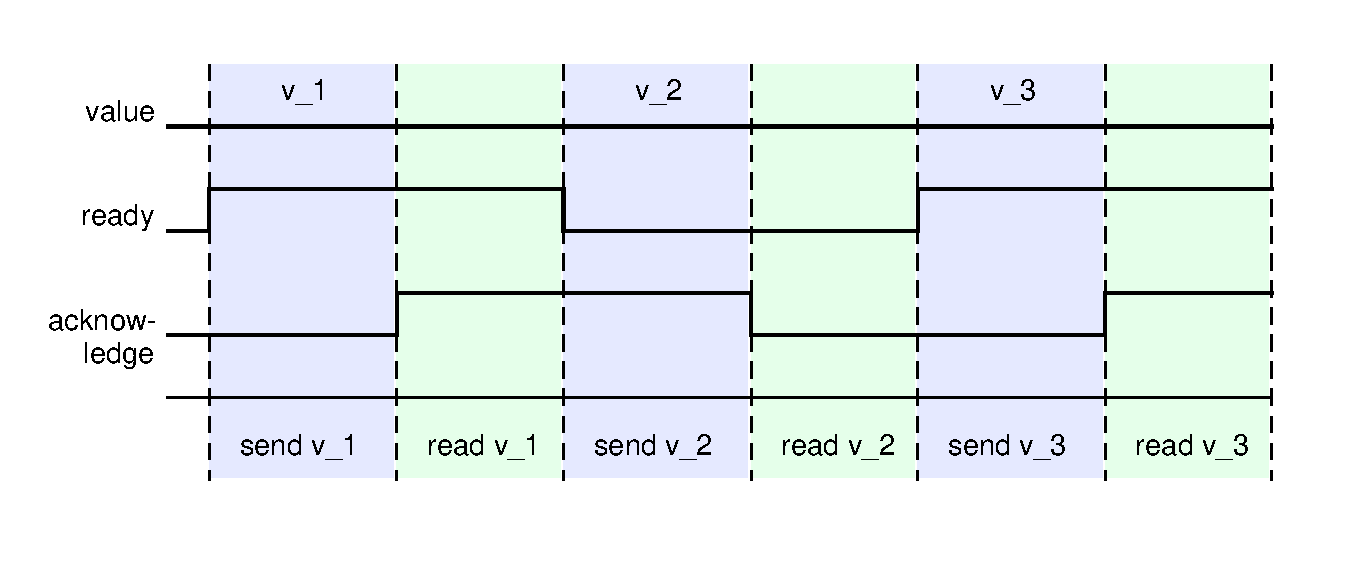
\includegraphics[scale=0.75]{Figures/AsyncInterface_send.pdf}
	\decoRule
	\caption{Asynchronous line transition states.}
	\label{fig:AsyncInterface_send}
\end{figure}

\section{Mathematical Specification Language (TLA\textsuperscript{+})}

The Formal Specification and Formal Design has to be written in a formal
mathematical language. CbyC suggests using Z  \parencite{CbyCPraxis}. 
I hound that Z has very little tool support and an inactive community. I decided
to use TLA\textsuperscript{+}.  TLA\textsuperscript{+} has frequently updated 
tooling and an active community. To get started with TLA\textsuperscript{+}
visit the ``Learning TLA\textsuperscript{+}'' website \parencite{LearningTLA}.

Using TLA\textsuperscript{+} we specify a system as a set of possible behaviours 
representing a correct execution of the system. We define a behaviour as a sequence
of states. A state is defined as an assignment of values to variables \parencite{SpecifyingSystems}.

\begin{figure}[H]
	\centering
	\includegraphics[scale=0.75]{Figures/System_Specification.pdf}
	\decoRule
	\caption{System specification.}
	\label{fig:SysSpec}
\end{figure}

In listing \ref{code:AsynchInterfaceSpec} we show the complete TLA specification of the 
asynchronous data interface. The TLA\textsuperscript{+} Toolbox can generate a 
pretty version as shown in figure \ref{fig:PDFCode}

The specification formula, \( Init \land \Box\left[ Next \right]_{\langle value, ready, acknowledge \rangle} \),
states that the initial state \(Init\) must be true at the start and that all 
subsequent states must be states specified in \(Next\).

\begin{lstlisting}[language = TLA, literate={-}{{-\allowbreak}}{1}, caption={Asynchronous data interface specification.}, captionpos=b, label={code:AsynchInterfaceSpec}]
--------------- MODULE AsynchInterface ---------------
EXTENDS Naturals
CONSTANTS Data
VARIABLES value, ready, acknowledge
TypeInvariant == /\ value \in Data
                 /\ ready \in {0,1}
                 /\ acknowledge \in {0,1}             
------------------------------------------------------
Init == /\ value \in Data
        /\ ready \in {0,1}
        /\ acknowledge = ready
        
Send == /\ ready = acknowledge
        /\ value' \in Data
        /\ ready' = 1 - ready
        /\ UNCHANGED acknowledge
        
Receive == /\ ready /= acknowledge
           /\ acknowledge' = 1 - acknowledge
           /\ UNCHANGED <<value, ready>>
              
Next == Send \/ Receive
Spec == Init /\ [][Next]_<<value, ready, acknowledge>>
------------------------------------------------------
THEOREM Spec => []TypeInvariant
======================================================
\end{lstlisting}

\begin{figure}[H]
	\centering
	\includegraphics[scale=0.75]{AsynchInterface_Code.png}
	\decoRule
	\caption{PDF code.}
	\label{fig:PDFCode}
\end{figure}

\section{Programming Language (C\#)}

CbyC suggests using the Ada SPARK programming language because it has native
support for code contracts and can verify the code using static analysis \parencite{CbyCPraxis}.
Very little line of business software is built using Ada. To make this more relevant 
to the my work I decided to use C\#. The problem with C\# is that is has no native
support for code contracts and also does not have sufficient static analysis tools 
capable of verifying code correct. This means that we will have to find workarounds
for these short comings. 

\subsection{Code Contracts}

CbyC program design is based on information flow expressed as code contracts 
\parencite{CbyCMan}. C\# does not have native code contracts any more \parencite{NoCodeContracts},
but it is very simple to implement code contracts using standard C\# language features.

Code contracts are an application of Hoare logic. Using Hoare logic
we can show that a program correctly implements a specification if, given a set of 
preconditions derived from the specification, the program never violates a set of
post conditions derived from the specification. We use the Hoare triple to 
represent the contract \parencite{BasisForProgramming}:

\[
	\{P\}Q\{R\}
\]

where:
\begin{description}
	\item [\(P\)] are the preconditions;
	\item [\(Q\)] is the program;
	\item [\(R\)] are the postconditions.
\end{description}

With some helper methods we can implement code contracts using standard C\# language
features. We are modelling our code contracts on the Design by Contract design 
\parencite{ObjectOrientedSoftwareConstruction}.

Design by Contract has two specification levels:
\begin{itemize}
	\item method preconditions and postconditions;
	\item class invariants.
\end{itemize}

Preconditions are a set of conditions that state what the method requires from 
the client (code calling the method) in order to function correctly.

Postconditions are a set of conditions that state what the method will ensure 
happens at the end of it's execution.

\lstset{style=sharpc, caption={Writing  code contracts using helper methods and classes.}}
\begin{lstlisting}[frame=single]
public int Method(...)
{
    //Preconditions
    Require(/*Consition*/, "Message")
        .Require(/*Consition*/, "Message");
        
    /// Method Code ...
    
    //Postconditions
    Ensure(/*Consition*/, "Message")
        .Ensure(/*Consition*/, "Message");

    return result;
}
\end{lstlisting}

Class invents are a set of conditions that will always be true after all 
executions.

\lstset{style=sharpc, caption={Writing  code contracts using helper methods and classes.}}
\begin{lstlisting}[frame=single]
public class Account
{
    ...

    public int Method(...)
    {
        /// Method Code ...
        ClassInvariant();
        return result;
    }
    
    private void ClassInvariant()
    {
        Invariant(/*Consition*/, "Message")
            .Invariant(/*Consition*/, "Message");
    }
}
\end{lstlisting}

\subsection{Verification}
Testing is usually the main method of verification and validation.  Unit testing
is inefficient because unit testing is ineffective and expensive. 
Unit testing is ineffective because most errors are interface errors, not internal
errors in units. Unit testing is expensive because you have to build test 
harnesses to test units in isolation \parencite{CbyCPraxis}.

Instead of unit testing code to show correctness we just want to verify 
that the contracts are not violated by the code are valid. When we know the 
code never violates the contracts we only need to create tests that show 
the different parts of the system function together.

We can represent a program or section of a program as a mathematical function
with all possible legal permutations of inputs seen as the function's domain and 
the output of the program the function's range.

It would be impractical to write unit tests that cover the complete input domain
of the program. Instead we write tests that take random points on the input domain
as input. We are not going to verify the outputs because if the outputs passes the 
contracts we assume the outputs are valid. This will eliminate the oracle problem 
\parencite{QuickCheck}.

When we tests smaller sections of the program separately random testing 
provides similar, adequate, code coverage as compared with determinisms testing
\parencite{QuickCheck}\parencite{Hamlet94randomtesting}.

We will be using FsCheck to create out property based tests. FsCheck is a .net 
implementation of QuickCheck \parencite{FsCheck_home}. 
